\documentclass{article}
\usepackage{fancyhdr}
\pagestyle{fancy}
\fancyfoot{}
\fancyfoot[C]{\thepage}
\rhead{Yarosevich - 1064712}
\usepackage{setspace}
\usepackage{siunitx} % Provides the \SI{}{} and \si{} command for typesetting SI units
\usepackage{graphicx} % Required for the inclusion of images
\usepackage{amsmath} % Required for some math elements 
\usepackage[export]{adjustbox} % loads also graphicx
\usepackage{listings}
\usepackage{setspace}
\usepackage{matlab-prettifier}
\usepackage{float}
\usepackage[most]{tcolorbox}
\usepackage{amsfonts}
\usepackage{color}
\usepackage{titlesec}
\usepackage{caption}
\usepackage{subcaption}
\usepackage{placeins}
\usepackage{bm}
\usepackage{esvect}
\newcommand{\uveci}{{\bm{\hat{\textnormal{\bfseries\i}}}}}
\newcommand{\uvecj}{{\bm{\hat{\textnormal{\bfseries\j}}}}}
\DeclareRobustCommand{\uvec}[1]{{%
  \ifcsname uvec#1\endcsname
     \csname uvec#1\endcsname
   \else
    \bm{\hat{\mathbf{#1}}}%
   \fi
}}


\newcommand{\R}{\mathbb{R}}

\usepackage{xcolor}

\DeclareCaptionFont{white}{\color{white}}
\DeclareCaptionFormat{listing}{%
  \parbox{\textwidth}{\colorbox{gray}{\parbox{\textwidth}{#1#2#3}}\vskip-4pt}}
\captionsetup[lstlisting]{format=listing,labelfont=white,textfont=white}
\lstset{frame=lrb,xleftmargin=\fboxsep,xrightmargin=-\fboxsep}
\titleformat{\section}[runin]
  {\normalfont\Large\bfseries}{\thesection}{1em}{}
\titleformat{\subsection}[runin]
  {\normalfont\large\bfseries}{\thesubsection}{1em}{}


\setlength\parindent{0pt} % Removes all indentation from paragraphs

\renewcommand{\labelenumi}{\alph{enumi}.} % Make numbering in the enumerate environment by letter rather than number (e.g. section 6)

%\usepackage{times} % Uncomment to use the Times New Roman font

%----------------------------------------------------------------------------------------
%	DOCUMENT INFORMATION
%----------------------------------------------------------------------------------------

\title{AMATH 503: Homework 3 \\Due April, 29 2019 \\ ID: 1064712} % Title

\author{Trent \textsc{Yarosevich}} % Author name

\date{\today} % Date for the report

\begin{document}
\maketitle % Insert the title, author and date
\setlength\parindent{1cm}

\begin{center}
\begin{tabular}{l r}
%Date Performed: December 1, 2017 \\ % Date the experiment was performed
Instructor: Ka-Kit Tung % Instructor/supervisor
\end{tabular}
\end{center}
\doublespacing
% If you wish to include an abstract, uncomment the lines below
% \begin{abstract}
% Abstract text
% \end{abstract}

%----------------------------------------------------------------------------------------
%	SECTION 1
%----------------------------------------------------------------------------------------
\section*{\textbf{(1)}}
To begin, we proceed with separation of variables as in class, assuming that the spatial component has to dependence on $\theta$. We thus assume a solution of the form:
\begin{equation}
\begin{aligned}
\Psi = T(t)u(r,z)
\end{aligned}
\end{equation}
When we apply this to the PDE we have:
\begin{equation}
\begin{aligned}
\frac{T''(t)}{c^2T(t)} = \frac{\nabla^2u}{u}
\end{aligned}
\end{equation}
We proceed as usual, noting that these ODEs must be equal to a constant, which we'll call $-\lambda^2$. This then gives the following solutions for the $T$ component:
\begin{equation}
\begin{aligned}
T(t) = Asin(c\lambda t) + Bcos(c\lambda t)
\end{aligned}
\end{equation}
From this equation we can then infer that the frequency is given by $\omega = c\lambda$, however this wavenumber $\lambda$ is determined by the spatial qualities of the cavity. Thus we move on to doing separation of variables of the spatial component, noting that we must apply the laplacian in cylindrical coordinates with no angular dependence:
\begin{equation}
\begin{aligned}
u(r,z) = R(r)Z(z)\\
\frac{Z''(z)}{Z(z)} + \frac{(rR'(r))'}{rR} = -\lambda^2\\ 
\end{aligned}
\end{equation}
We now assume the $Z$ component is equal to some constant $-b^2$, giving the familiar family of solutions to which we can apply some boundary conditions:
\begin{equation}
\begin{aligned}
\frac{Z''(z)}{Z(z)} = -b^2\\
Z(z) = A_lsin(bz) + B_lcos(bz)\\
Z(0) = 0 = B_l\\
Z(L) = 0 = A_lsin(bL)\\
bL = l\pi\\
b = \frac{l\pi}{L}\\
l = 1,2,3...
\end{aligned}
\end{equation}
Now that we know the value of $b$ (or $b_l$), we have the following:
\begin{equation}
\begin{aligned}
\frac{(rR'(r))'}{rR} +(\lambda^2 - b^2) = 0\\ 
(rR'(r))' + rR(\lambda^2 - b^2) = 0\\
rR''(r) + R'(r) + rR(\lambda^2 - b^2) = 0\\ 
\end{aligned}
\end{equation}
So now we want to put this in the form of Bessel's equation. We do this by multiplying through by $r$ and substituting $x = r\sqrt{\lambda^2-b^2}$ and $y(x) = R(r)$ as in the notes, section (11.22). 
\begin{equation}
\begin{aligned}
r^2R''(r) + rR'(r) + r^2R(\lambda^2 - b^2) = 0\\ 
x^2y''(x) + xy'(x) + x^2y(x) = 0
\end{aligned}
\end{equation}
In lecture, the Professor noted that once we get to this standard form for the Bessel equation, we should proceed directly to the solution obtained by the Frobenius expansion, $y(x) = AJ_m(x) + BY_m(x)$. However, we can immediately note that the solution is bounded at $R(0)$, and so we have a Bessel function of he first kind, with $B=0$, since $Y_m(x)$ blows up at $x=0$. We thus have:
\begin{equation}
\begin{aligned}
y(x) = AJ_m(x)\\
R(r) = AJ_m(r\sqrt{\lambda^2 - b^2})
\end{aligned}
\end{equation}
Applying the other boundary condition that $\Psi = 0$ at $r=a$, we require $R(a) = AJ_m(a\sqrt{\lambda^2 - b^2}) = 0$. The zeros $z_{mn}$ of of the Bessel function are tabulated on page 146 of the notes, thus we must require that $a\sqrt{\lambda^2 - b ^2} = z_{mn}$. Solving for $\lambda^2$:
\begin{equation}
\begin{aligned}
a\sqrt{\lambda^2 - b ^2} = z_m\\
(\frac{z_{mn}}{a})^2 = \lambda^2 - b^2\\
\lambda^2 = (\frac{z_{mn}}{a})^2 + b^2
\end{aligned}
\end{equation}
We can now refer back to the fact that $\omega=c\lambda$, and substitute in the value for $b$, giving the following:
\begin{equation}
\begin{aligned}
\lambda = \sqrt{(\frac{z_{mn}}{a} + (\frac{l\pi}{L})^2}\\
\omega = c\sqrt{(\frac{z_{mn}}{a} + (\frac{l\pi}{L})^2}\\
\end{aligned}
\end{equation}
Plugging in our values in the prompt, and noting that $1cm^2 = .0001m^2$, we have:
\begin{equation}
\begin{aligned}
w_{nl} = \frac{300m}{s}\sqrt{(\frac{z_{mn}^2}{.0001m^2}) + (\frac{l^2\pi^2}{.5m^2})}\\
\end{aligned}
\end{equation}
Now, it is immediately clear that $z_{nm}$ contributes far more to the frequency than the $l$ term, since it is divided by a number three orders of magnitude smaller, thus the lowest frequencies will be given by $z_{1,0}$ and $l=1,2,3$. Dividing by $2\pi$ to convert to Hz, we have:
\begin{tcolorbox}[minipage,colback=white,arc=0pt,outer arc=0pt]
\begin{equation}
\begin{aligned}
w_{1,1} = 72.169\frac{rad}{sec} \to 11.486 \text{ kHz}\\
w_{1,2} = 72.243\frac{rad}{sec} \to 11.498 \text{ kHz}\\
w_{1,3} = 72.366\frac{rad}{sec} \to 11.517 \text{ kHz}\\
\end{aligned}
\end{equation}
\end{tcolorbox}
\section*{\textbf{(2)}}
To find the energy levels we have to solve for the eigenvalues in the spatial component, i.e. we need to solve a spherical Bessel's equation. Again we proceed by separation of variables, noting that there is no angular component, and substitute our assumed form into the PDE:
\begin{equation}
\begin{aligned}
\Psi = T(t)u(r)\\
\frac{ihT'(t)}{T(t)} = \frac{-h^2}{2\mu}\frac{\nabla^2u}{u} = E\\
T(t) = T(0)e^{-\frac{i}{h}t}\\
\end{aligned}
\end{equation}
$E$ is interpreted as the energy of the electron, as noted in section 11.2 of the notes, since $\frac{E}{h}$ is the frequency of the electron and $h$ times the frequency is the energy of the electron. Moving on to the spatial component we have the laplacian in spherical coordinates with no angular dependence, plus some constants $\lambda^2 = \frac{2\mu E}{h^2}$, giving:
\begin{equation}
\begin{aligned}
\nabla^2u = \frac{1}{r^2}\frac{d}{dr}(r^2\frac{d}{dr}u) = -\lambda^2u\\
u(r) = R(r)\\
R''(r) + \frac{2R'(r)}{r} + R\lambda^2 = 0
\end{aligned}
\end{equation}
We now want to try to put this in the form of a Bessel function by multiplying through by $r^2$ and letting $x=\lambda r$ and $R(r) = \frac{w(x)}{x}$ as given in section (11.36) of the notes. First, we must determine $R''(r)$ and $R'(r)$:
\begin{equation}
\begin{aligned}
x^2\frac{d^2}{dx^2}R + 2x\frac{d}{dx}R + x^2R = 0\\
\frac{d}{dx}R = -x^{-2}w(x) + x^{-1}{w'(x)}\\
\frac{d^2}{dx^2} = 2x^{-3}w(x) - x^{-2}w'(x) - x^{-2}w'(x) + x^{-1}w''(x)\\
\frac{d^2}{dx^2} = 2x^{-3}w(x) - 2x^{-2}w'(x) + x^{-1}w''(x)\\
\end{aligned}
\end{equation}
Substituting into our spherical Bessel function:
\begin{equation}
\begin{aligned}
x^2 \Big{[} 2x^{-3}w(x) &- 2x^{-2}w'(x) + x^{-1}w''(x) \Big{]}\\
 &+ 2x \Big{[}-x^{-2}w(x) + x^{-1}{w'(x)} \Big{]} + x^2(x^{-1}w(x)) = 0\\
\end{aligned}
\end{equation}
\begin{equation}
\begin{aligned}
 2x^{-1}w(x) - 2w'(x) + xw''(x) - 2x^{-1}w(x) + 2xw'(x) + xw(x) = 0\\
 x(w''(x) + w(x)) = 0\\
 w(x) = Asin(x) + Bcos(x)
\end{aligned}
\end{equation}
Substituting back $R(r) = \frac{w(x)}{x}$:
\begin{equation}
\begin{aligned}
R(r) = A\frac{sinx}{x} + B\frac{cosx}{x}
\end{aligned}
\end{equation}
We then note the equation must be bounded at $x=0$ so we can't have it blowing up. As a result $B=0$. We could use L'Hospital's rule with the remaining term, but I'm going to go with a snarky reddit mathematician and simply note that if we know $\frac{d}{dx}sinx = cosx$ and $cos(0) = 1$ then as $x\to$, the fraction $\frac{sinx}{x}$ must be 1. Thus this term is still bounded at $x=0$. Applying the other BC $\Psi=0$ at $r=a$ we have:
\begin{equation}
\begin{aligned}
R(a) = A\frac{sin(\lambda a)}{\lambda a})
\end{aligned}
\end{equation}
The resulting non-trivial solution requires that $\lambda = \lambda_k=\frac{k\pi}{a}$ with $k=1,2,3...$. So we have our value for $\lambda$, which we can plug back into the substitution in \textbf{(14)} above giving:
\begin{tcolorbox}[minipage,colback=white,arc=0pt,outer arc=0pt]
\begin{equation}
\begin{aligned}
\lambda^2 = \lambda_k^2 = (\frac{k\pi}{a})^2 =  \frac{2\mu E}{h^2}\\
E = E_k = \frac{(k\pi h)^2}{2a^2\mu}\\
k = 1,2,3...
\end{aligned}
\end{equation}
\end{tcolorbox}
\section*{\textbf{(3)}}
\subsection*{\textbf{($a_0$ and $P_0$)}}
First, we have $P_0=1$ from the notes. To calculate $a_0$ we use the formula:
\begin{equation}
\begin{aligned}
a_0 = \frac{1}{2}\int_0^1xdx = \frac{1}{2}[\frac{x^2}{2}]\Big{|}^1_0 = \frac{1}{4}
\end{aligned}
\end{equation}
\subsection*{\textbf{($a_1$ and $P_1$)}}
By Rodrigue's Formula:
\begin{equation}
\begin{aligned}
P_1 = \frac{1}{2}\frac{d}{dx}(x^2-1) = x\\
a_1 = \frac{3}{2}\int_0^1x^2dx = \frac{1}{2}[\frac{x^2}{3}]\Big{|}^1_0 = (\frac{3}{2})(\frac{1}{3}) = \frac{1}{2}
\end{aligned}
\end{equation}
\subsection*{\textbf{($a_2$ and $P_2$)}}
\begin{equation}
\begin{aligned}
P_2 = \frac{1}{2!}\frac{d^2}{dx^2}(x^2-1)^2\\
\frac{d}{dx}(x^2-1)^2 = 2(2x)(x^1-1) \\
\frac{d}{dx}2(2x)(x^1-1) = 12x^2-4\\
P_2 = \frac{1}{8}(12x^2-4) = \frac{3}{2}x^2 - \frac{1}{2}
\end{aligned}
\end{equation}
\begin{equation}
\begin{aligned}
a_2 = \frac{5}{2}\int_0^1\frac{3}{2}x^2 - \frac{1}{2}dx\\
a_2 = \frac{5}{2}\Big{[}\int_0^1\frac{3x^2}{2}dx - \int_0^1\frac{x}{2}dx \Big{]}\\
a_2 = \frac{5}{2}\Big{[}[\frac{3x^4}{8}]\Big{|}_0^1 - [\frac{x^2}{4}]\Big{|}_0^1 \Big{]}\\
a_2 = \frac{5}{2} (\frac{3}{8} - \frac{1}{4}) = \frac{5}{16}
\end{aligned}
\end{equation}
\subsection*{\textbf{($a_3$ and $P_3$)}}
\begin{equation}
\begin{aligned}
P_3 = \frac{1}{8(3!)}\frac{d^3}{dx^3}(x^2-1)^3\\
\frac{d}{dx}(x^2-1)^3 = 6x(x^2)^2\\
\frac{d}{dx}6x(x^2)^2 = 6(x^2-1)^2 + 24x^2(x^2-1)\\
\frac{d}{dx}6(x^2-1)^2 + 24x^2(x^2-1) = 24x(x^2-1) + 96x^3-48x\\
P_3 = \frac{1}{48}(24x^3 - 24x +96x^3-48x)= \frac{5}{2}x^3 - \frac{3}{2}x
\end{aligned}
\end{equation}
\begin{equation}
\begin{aligned}
a_3 = \frac{35}{4}\int_0^1x^4dx - \frac{21}{4}\int_0^1x^2dx\\
a_3 = \frac{35}{4}(\frac{1}{5}) - \frac{21}{4}(\frac{1}{3}) = 0
\end{aligned}
\end{equation}
\subsection*{\textbf{($a_4$ and $P_4$)}}
Since $a_3=0$, we'll continue in order to get a fourth non-zero term. Strap in!
\begin{equation}
\begin{aligned}
P_4 = \frac{1}{2^4(4!)}\frac{d^4}{dx^4}(x^2-1)^4\\
\frac{d}{dx}(x^2-1)^4 = 8x(x^2-1)^3\\
\frac{d}{dx} 8x(x^2-1)^3 = 8(x^2-1)^3+48x^2(x^2-1)^2\\
\frac{d}{dx} 8(x^2-1)^3+48x^2(x^2-1)^2 = 24(2x)(x^2-1)^2 + 96x(x^2-1)^2 + 48x^2(4x)(x^2-1)\\
\frac{d}{dx} 8(x^2-1)^3+48x^2(x^2-1)^2 = 144x(x^2-1)^2+192x^5-192x^3\\
144x(x^2-1)(x^2-1)+192x^5-192x^3 = 144x^5-288x^3+144x+192x^5-192x^3\\
144x^5-288x^3+144x+192x^5-192x^3 = 336x^5 - 480^3 + 144x\\
\frac{d}{dx}336x^5 - 480^3 + 144x=1680x^4 - 1440x^2+144\\
P_4 = \frac{1}{384}(1680x^4 - 1440x^2+144) = \frac{35}{8}x^4 - \frac{15}{4}x^3+\frac{3}{8}
\end{aligned}
\end{equation}
\begin{equation}
\begin{aligned}
a_4 = \frac{9}{2} \Big{[} \frac{35}{8}\int_0^1x^5dx - \frac{15}{4}\int_0^1x^3dx +\frac{3}{8}\int_0^1xdx \Big{]}\\
a_4 =\frac{316}{16}(\frac{1}{6}) - \frac{135}{8}(\frac{1}{4}) + \frac{27}{16}(\frac{1}{2}) = \frac{-3}{32}
\end{aligned}
\end{equation}
To summarize, we have the following non-zero values:
\begin{tcolorbox}[minipage,colback=white,arc=0pt,outer arc=0pt]
\begin{equation}
\begin{aligned}
a_0 = \frac{1}{4}\text{ , } & P_0 = 1\\
a_1 = \frac{1}{2}\text{ , } & P_1 = x\\
a_2 = \frac{5}{16}\text{ , } & P_2 = \frac{3}{2}x^2-\frac{1}{2}\\
a_4 = \frac{-3}{32}\text{ , } & P_4 = \frac{35}{8}x^4 - \frac{15}{4}x^2 +\frac{3}{8}\\
\end{aligned}
\end{equation}
\end{tcolorbox}
Below are the plots of one, two, three, and all four, terms:
    \begin{figure*}
        \centering
        \begin{subfigure}[b]{0.8\textwidth}
            \centering
            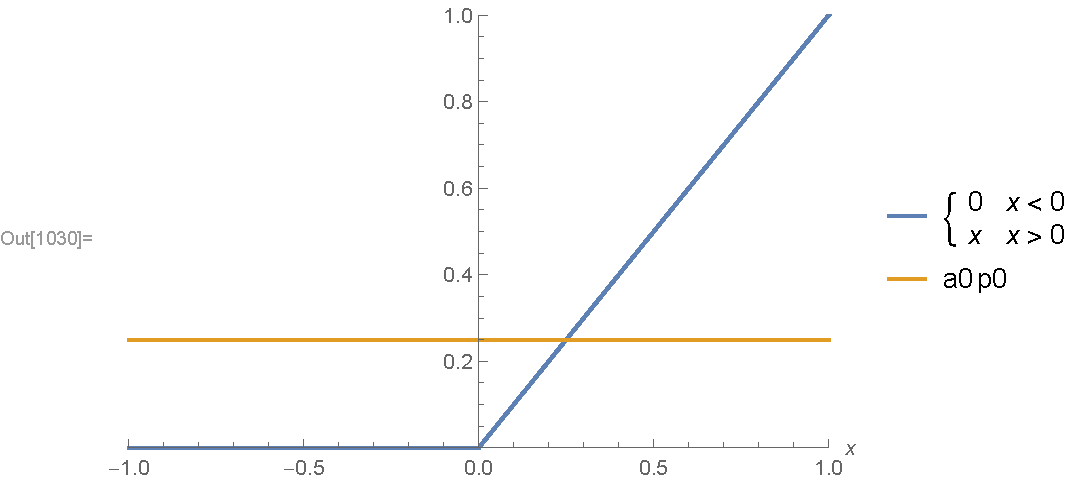
\includegraphics[width=\textwidth]{part3_a0.pdf}
            %\caption[Network2]%
            %{{\small Network 1}}    
            %\label{fig:mean and std of net14}
        \end{subfigure}
        \hfill
        \begin{subfigure}[b]{0.8\textwidth}  
            \centering 
            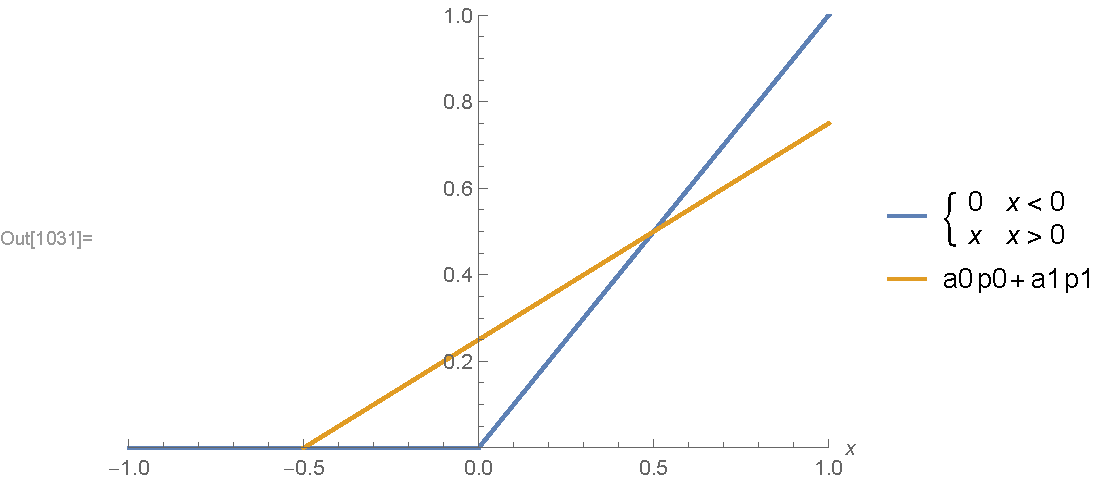
\includegraphics[width=\textwidth]{part3_a1.pdf}
            %\caption[]%
            %{{\small Network 2}}    
            %\label{fig:mean and std of net24}
        \end{subfigure}
        \vskip\baselineskip
        \begin{subfigure}[b]{0.8\textwidth}   
            \centering 
            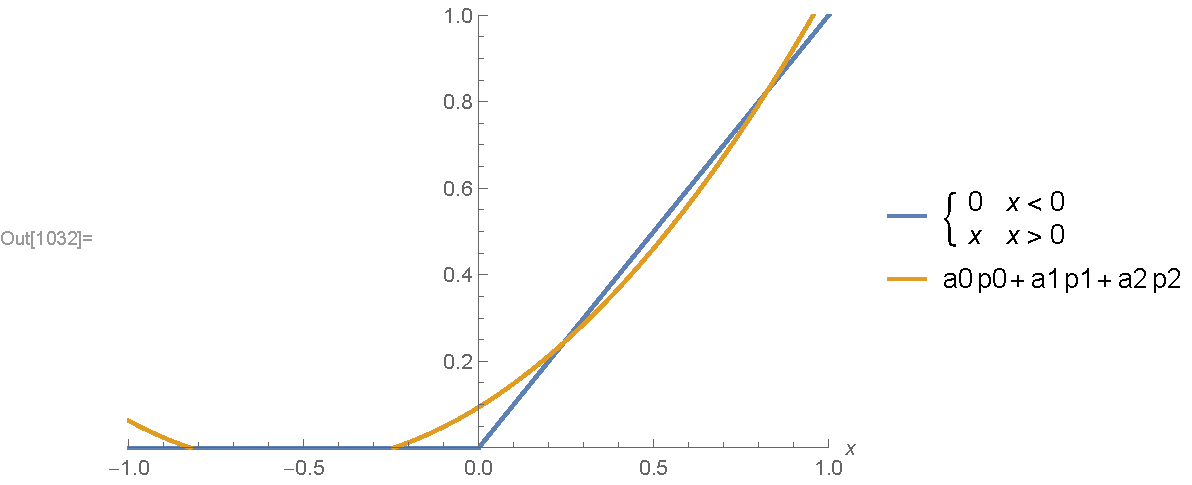
\includegraphics[width=\textwidth]{part3_a2.pdf}
            %\caption[]%
            %{{\small Network 3}}    
            %\label{fig:mean and std of net34}
        \end{subfigure}
        \quad
        \begin{subfigure}[b]{0.8\textwidth}   
            \centering 
            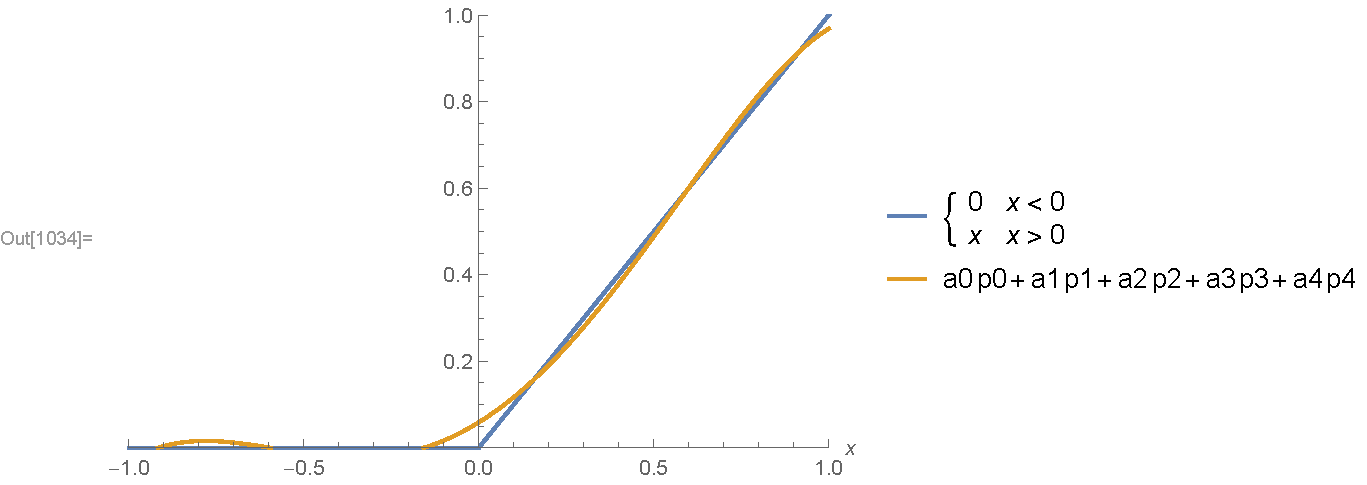
\includegraphics[width=\textwidth]{part3_a4.pdf}
            %\caption[]%
            %{{\small Network 4}}    
            %\label{fig:mean and std of net44}
        \end{subfigure}
        %\caption[ The average and standard deviation of critical parameters ]
        %{\small The average and standard deviation of critical parameters: Region R4} 
        %\label{fig:mean and std of nets}
    \end{figure*}


\end{document}